\begin{thm}{217}{\hosi 6}{一橋 (2018)}
 $f(x)=\dfrac{x^2-1}{2}$とおく。$-1\le t \le 1$とし、曲線$y=f(x)$上の点$\left(t,f(t)\right)$における接線を$L$とする。半円$x^2+y^2=1$ $(y\le 0)$ と$L$で囲まれた部分の面積を$S$とする。$S$の取り得る値の範囲を求めよ。
\end{thm}

\begin{figure}[H]
 \centering
 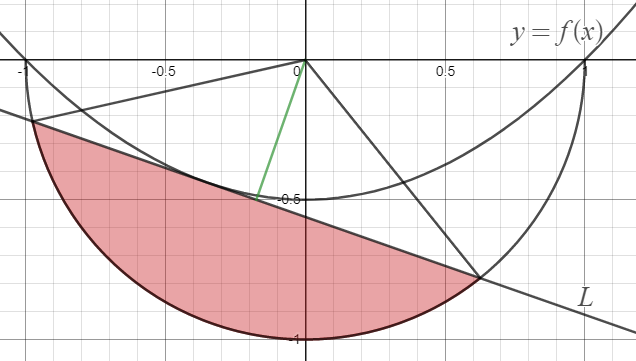
\includegraphics[width=0.7\linewidth]{../problems/Q_217/A_217.png}
\end{figure}

$f'(x)=x$であるから、接線$L$の方程式は$y=tx-\dfrac{t^2+1}{2}$となる。これと原点との距離$d$は、$d=\dfrac{\left|t\cdot 0-0-\frac{t^2+1}{2}\right|}{\sqrt{t^2+1}}=\dfrac{\sqrt{t^2+1}}{2} < 1$であり、かつ点$(\pm1, 0)$は接線$L$上にあるかこれより上にあるので、接線と半円の弧は常に2点で交わる。

よって領域は常に半円と$L$ (が半円に切り取られる弦) のみに囲まれており、その面積は$L$と原点との距離$d=\dfrac{\sqrt{t^2+1}}{2}$が長いほ
ど小さくなり、短いほど大きくなる。

$d$が最大となるのは$t=\pm 1$のときで、$d=\dfrac{1}{\sqrt{2}}$。このとき面積は最小で、その値は下左図より$S=\dfrac{\pi}{4}-\dfrac{1}{2}$。

$d$が最小となるのは$t=0$のときで、$d=\dfrac{1}{2}$。このとき面積は最大で、その値は下右図より$S=\dfrac{\pi}{3}-\dfrac{\sqrt{3}}{4}$。

\begin{figure}[H]
 \centering
 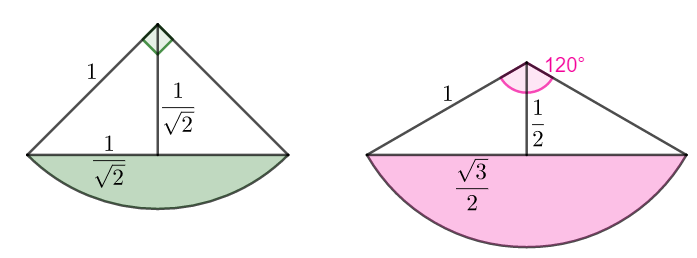
\includegraphics[width=0.6\linewidth]{../problems/Q_217/A_217_2.png}
\end{figure}

以上より、$S$の取り得る範囲は$\dfrac{\pi}{4}-\dfrac{1}{2}\le S \le \dfrac{\pi}{3}-\dfrac{\sqrt{3}}{4}$